\chapter{結論}
\section{本研究の成果}
%と,限定された点を明らかにしたり,
%さらに改善されるべき点を述べる

以上の通り,スマートデバイスを用いて
DBAP法を用いたスピーカアレイを構築できることを示した.


\section{本研究の展望}
%どうしたらもっとよくなるか
%どうしたら残ってる問題を解決できそうか.

\subsection{相対位置推定結果が回転・反転する問題}



ダイレクトパスがない時に同期性能落ちる.
端末間に障害物があると音波が回折して伝搬する.
コンクリート壁などの反射波の方がエネルギー大きくなる、あるいは非線形歪みの影響がある\cite{nonlinear}.
微弱な先行波を捉える手法の必要性があるが,非線形歪みと反射音,回折音をどう区別するかの問題が残っている.
ハードウェアや環境に応じて2端末間のインパルス応答は毎回異なるため識別は困難である.


\subsection{相対位置推定結果が回転・反転する問題}

相対位置推定の結果が理解できない.
問題設定上,回転や鏡面反転した解が出てきてしまう.
これは,相対位置を推定している以上防ぐことができない.
そのため,ユーザが手で修正するためのUIを実装する必要がある.
他にも,2台の端末の位置を固定してしまい推定から外してしまえば,回転・反転は防ぐことができる.


\subsection{相対位置推定アルゴリズムの解が収束していない}

相対位置推定の結果が現実の位置を反映できていない.
これは,最急降下法の解が収束していないのが原因である.
推定アルゴリズムを改良する必要がある.


\subsection{音圧校正}

端末ごとに音圧出力が異なる問題もある.
これは,スピーカアンプの出力の差が原因である.
これには,互いに観測したパルスの振幅から距離減衰を推定し,相対的な音圧比率を計算することができる.
(図:\ref{fig:spc})

\begin{figure}[p]
  \centering
  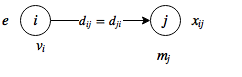
\includegraphics[clip,width=1.05\hsize]{img/sound_pressure_calibration.png}
  \caption{2端末間の振幅減衰のモデル}\label{fig:spc}
\end{figure}

$$
ev_i \frac{1}{d_{ij}}m_j = x_{ij}
$$

$$
\frac{v_j}{v_k} = \frac{x_{ij}d_{ij}}{x_{kj}d_{kj}}
$$

これもこのモデルが成り立つか実験が必要である.


\subsection{システムクロックの校正}

システムクロックの差に依存するズレがある.
これを解決するには2端末間でシステムクロックの差を検出すればよい.
具体的には2回パルス受信してサンプリング数の差を計測すれば良い(図\ref{fig:ps2}).

$$
\frac{S_B}{S_A} = \frac{i+d}{i}
$$

\begin{figure}[p]
  \centering
  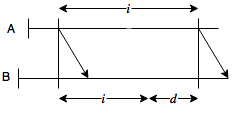
\includegraphics[clip,width=1.05\hsize]{img/phase_shift2.png}
  \caption{再同期}\label{fig:ps2}
\end{figure}

\subsection{パルス検出できない端末間で同期}
多段同期すればよい
クロック校正も多段校正できる
音圧校正も多段校正できる(図\ref{fig:nt})

\begin{figure}[p]
  \centering
  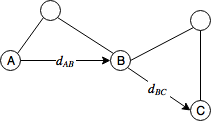
\includegraphics[clip,width=1.05\hsize]{img/network_topology.png}
  \caption{再同期1}\label{fig:nt}
\end{figure}



端末 $A$ を基準に音圧校正を考えると

$$
\frac{v_B}{v_A} = \frac{x_{iB} d_{iB}}{x_{AB}d_{AB}} \\
\frac{v_C}{v_B} = \frac{x_{iC} d_{iC}}{x_{BC}d_{BC}} \\
$$

であるので

$$
\frac{v_C}{v_A} =
\frac{v_B v_C}{v_A v_B} =
\frac{x_{iB} x_{iC} d_{iB} d_{iC}}{x_{AB} x_{BC} d_{AB} d_{BC}}
$$

とすれば端末 A と端末 C の出力比率を求められる.
要実験である.

また,同期に関しては,
時刻の基準となる
端末 $A$ がパルスを発した時間を $t_{AA}$ として
そのパルスが端末 $B$ に届いた時間は $t_{AB}$ とする.
また,
端末 $B$ がパルスを発した時間を $t_{AB}$ として
そのパルスが端末 $C$ に届いた時間は $t_{BC}$ とする.
そしてそれぞれの伝達時間を $d$ とすると図\ref{fig:rd}のようになる.

\begin{figure}[p]
  \centering
  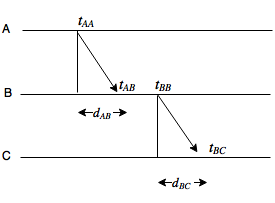
\includegraphics[clip,width=1.05\hsize]{img/rel_delay.png}
  \caption{再同期2}\label{fig:rd}
\end{figure}

このとき,まず端末 $C$ は端末 $B$ と同期して,
その後端末 $B$ と端末 $A$ の時刻ずれ情報をもとにさらに端末 $A$ との同期ができる.



\subsection{パルス回数の問題}
現在の提案手法では同期に時間がかかるのでリアルタイム同期できるようにしたい.
N台の同期にN回パルス必要という問題もある.
これには,TDMAだけでなくCDMA(符号分割多元接続)も試した.
シミュレーションではうまく機能したが,
実際に試すとパルスが重なったときに信号をうまく分離できない問題があった.
これも拡散符号の非線形歪みの影響と考えられる.
ところで,音圧校正・同期を考えなければ,つまり測距だけならば,パルスは3台が1回ずつ放てば十分である.
これはGPSと同じ仕組みであり,3台の端末の相対位置さえわかってしまえば,
他の端末はその3台からの相対距離がわかれば三角測量の要領で相対位置が算出できるからである.
この手法に合わせて同期手法を提案手法とは異なる結合振動子系のような適応的アルゴリズムにすることで,システムクロックのずれにも対応できるようになる.
しかしながら,音圧校正のためには現在の手法では全ての端末が音を出す必要がある問題が残されている.


\subsection{位置変更による再同期の必要性}

端末が動くと再同期が必要という問題もある.
この原因は同期と測距を同時にしているからである.
逆に言えば,測距と同期とは別の手法を用いればよい.
例えば,GPSと同じように,位置固定した連続パルス発信端末を導入すればよい.
これにより,リアルタイム測距は可能になる.
同期に関してはも結合振動子系のような適応的なアルゴリズムを採用すれば,システムクロックのずれにも対応できるようになる
しかしながら,音圧校正のためには現在の手法では全ての端末が音を出す必要がある問題が残されている.


\subsection{計算量・計算時間削減のための最適化}
相互相関の計算に離散フーリエ変換ではなく離散コサイン変換を使うことで計算量を削減できる可能性がある.
しかしながら,高速離散フーリエ変換を高速離散コサイン変換に置き換えたことによる計算量の削減は高々O(n)であり、負荷改善のために導入するには最適化の時期が早すぎると思われる.


\section{本研究の総括と結論}

教室空間における複数の個人所有のスマートデバイスを用いてスピーカアレイを構築し,DBAP法を用いた音像定位するシステムを提案した・
各端末を音声パルスを用いることで時刻同期し,位置を推定し,仮想音源を配置できることを示した.
これにより教室空間における新しい音声コミュニケーション手法を実現した.
